\documentclass[unicode,11pt,a4paper,oneside,numbers=endperiod,openany]{scrartcl}

% Required package
\usepackage{amssymb}
\usepackage{graphicx}
\usepackage{amsmath}
\usepackage{matlab-prettifier}
\usepackage{float}
\usepackage[export]{adjustbox}
\usepackage{multirow}

\renewcommand{\thesubsection}{\arabic{subsection}}

% vector shortcut
\newcommand{\myvec}[1]{\begin{bmatrix} #1 \end{bmatrix}}
\newcommand{\myex}[1]{\begin{equation*}\begin{aligned} #1 \end{aligned}\end{equation*}}
\newcommand{\myexthreeA}{\myvec{2 & 0 \\ 0 & 2\mu}}

\usepackage{ifthen}
\usepackage[utf8]{inputenc}
\usepackage{graphics}
\usepackage{graphicx}
\usepackage{hyperref}
\usepackage{amsmath}

\pagestyle{plain}
\voffset -5mm
\oddsidemargin  0mm
\evensidemargin -11mm
\marginparwidth 2cm
\marginparsep 0pt
\topmargin 0mm
\headheight 0pt
\headsep 0pt
\topskip 0pt        
\textheight 255mm
\textwidth 165mm

\newcommand{\duedate} {}
\newcommand{\setduedate}[1]{%
\renewcommand\duedate {\textbf{Due date:}~ #1}}
\newcommand\isassignment {false}
\newcommand{\setassignment}{\renewcommand\isassignment {true}}
\newcommand{\ifassignment}[1]{\ifthenelse{\boolean{\isassignment}}{#1}{}}
\newcommand{\ifnotassignment}[1]{\ifthenelse{\boolean{\isassignment}}{}{#1}}

\newcommand{\assignmentpolicy}{
\begin{table}[h]
\begin{center}
\scalebox{0.8} {%
\begin{tabular}{|p{0.02cm}p{16cm}|}
\hline
&\\
\multicolumn{2}{|c|}{\Large\textbf{Numerical Computing 2023 ---  Submission Instructions}}\\
\multicolumn{2}{|c|}{\large\textbf{(Please, notice that following instructions are mandatory: }}\\
\multicolumn{2}{|c|}{\large\textbf{submissions that don't comply with, won't be considered)}}\\
&\\
\textbullet & Assignments must be submitted to \href{https://www.icorsi.ch/course/view.php?id=14666}{iCorsi} (i.e. in electronic format).\\
\textbullet & Provide both executable package and sources (e.g. C/C++ files, MATLAB). 
If you are using libraries, please add them in the file. Sources must be organized in directories called:\\
\multicolumn{2}{|c|}{\textit{Project\_number\_lastname\_firstname}}\\
& and  the  file must be called:\\
\multicolumn{2}{|c|}{\textit{project\_number\_lastname\_firstname.zip}}\\
\multicolumn{2}{|c|}{\textit{project\_number\_lastname\_firstname.pdf}}\\
\textbullet &  The TAs will grade your project by reviewing your project write-up, and looking at the implementation you attempted, and benchmarking your code's performance.\\

\textbullet & You are allowed to discuss all questions with anyone you like; however: (i) your submission must list anyone you discussed problems with and (ii) you must write up your submission independently.\\
\hline
\end{tabular}
}
\end{center}
\end{table}
}
\newcommand{\punkte}[1]{\hspace{1ex}\emph{\mdseries\hfill(#1~\ifcase#1{Points}\or{Points}\else{Points}\fi)}}


\newcommand\serieheader[6]{
\thispagestyle{empty}%
\begin{flushleft}

\includegraphics[width=0.45\textwidth]{CI_logo}
\end{flushleft}
  \noindent%
  {\large\ignorespaces{\textbf{#1}}\hspace{\fill}\ignorespaces{ \textbf{#2}}}\\ \\%
  {\large\ignorespaces #3 \hspace{\fill}\ignorespaces #4}\\
  \noindent%
  \bigskip
  \hrule\par\bigskip\noindent%
  \bigskip {\ignorespaces {\Large{\textbf{#5}}}
  \hspace{\fill}\ignorespaces \large \ifthenelse{\boolean{\isassignment}}{\duedate}{#6}}
  \hrule\par\bigskip\noindent%  \linebreak
 }

\makeatletter
\def\enumerateMod{\ifnum \@enumdepth >3 \@toodeep\else
      \advance\@enumdepth \@ne
      \edef\@enumctr{enum\romannumeral\the\@enumdepth}\list
      {\csname label\@enumctr\endcsname}{\usecounter
        {\@enumctr}%%%? the following differs from "enumerate"
	\topsep0pt%
	\partopsep0pt%
	\itemsep0pt%
	\def\makelabel##1{\hss\llap{##1}}}\fi}
\let\endenumerateMod =\endlist
\makeatother




\usepackage{textcomp}





\begin{document}


\setassignment
\setduedate{Tuesday, 19 March 2024, 12:00 AM}

\serieheader
{Optimization Methods}
{2024}
{\textbf{Student:} Jeferson Morales Mariciano \\\\}
{\textbf{Discussed with:} Leonardo Birindelli}
{Assignment 1}{}
\newline

%\assignmentpolicy


% EXERCISE 1 %%%%%%%%%%%%%%%%%%%%%%%%%%%%%%%%%%%%%%%%%%%%%%%%%%%%%%%%%%%%%%%%%%%%%%%%%%%%%%%%%%%%%%
\section{Exercise 1}
Vector-valued function $f : \mathbb{R}^2 \rightarrow \mathbb{R}$

\begin{equation}
    f(x_1, x_2) = 200 (x_2 - x_1^2)^2 + (1 - x_1)^2
\end{equation}

\subsection{}
Compute gradient $\nabla f : \mathbb{R}^2 \rightarrow \mathbb{R}^2$
and Hessian $H_f : \mathbb{R}^2 \rightarrow \mathbb{R}^{2 \times 2}$. \newline

\begin{equation*}
\begin{aligned}
    \begin{bmatrix} x_1 \\ x_2 \end{bmatrix}
     & \mapsto 200 (x_2 - x_1^2) (x_2 - x_1^2) + (1 - x_1) (1 - x_1) \\
     & = 200 (x_2^2 - 2x_2 x_1^2 + x_1^4) + (1 - 2x_1 + x_1^2)       \\
     & = 200 x_2^2 - 400 x_2 x_1^2 + 200 x_1^4 + 1 - 2x_1 + x_1^2    \\
    \nabla f
     & = \begin{bmatrix}
             \frac{\partial f}{\partial x_1} \\
             \frac{\partial f}{\partial x_2}
         \end{bmatrix}
    = \begin{bmatrix}
          -800 x_2 x_1 + 800 x_1^3 + 2x_1 - 2 \\
          400 x_2 - 400 x_1^2
      \end{bmatrix} \\
    H_f
     & =\begin{bmatrix}
            \frac{\partial^2 f}{\partial x_1^2}            
            & \frac{\partial^2 f}{\partial x_1 \partial x_2} \\
            \frac{\partial^2 f}{\partial x_2 \partial x_1} 
            & \frac{\partial^2 f}{\partial x_2^2}            \\
        \end{bmatrix}
    = \begin{bmatrix}
          -800 x_2 + 2400 x_1^2 + 2 & - 800 x_1 \\
          -800 x_1                  & 400
      \end{bmatrix}
\end{aligned}
\end{equation*}

\subsection{}
Write Taylor's expansion of $f$ up to 2nd order around point
$(x_1, x_2) = (0, 0)$. \newline

Given $x_0 = (0, 0)$, $f(x_0) = 1$, 
$\nabla f(x_0) = \begin{bmatrix} -2 \\ 0 \end{bmatrix}$, 
$H_f(x_0) = \begin{bmatrix} 2 & 0 \\ 0 & 400 \end{bmatrix}$, 
incognites $h = \begin{bmatrix} x_1 \\ x_2 \end{bmatrix}$

\begin{equation*}
\begin{aligned}
    f(x_0 + h)
     & = f(x_0) + h^T \nabla f(x_0) + \frac{1}{2} h^T H_f(x_0) h + o(|| h ||^2)                                                                                                                                                                                                                                                                                      \\
     & = 1 + \myvec{x_1 & x_2} \myvec{-2 \\ 0 } + \frac{1}{2} \myvec{x_1 & x_2} \myvec{2 & 0 \\ 0 & 400} \myvec{x_1 \\ x_2} + o(|| h ||^2) \\
     & = 1 - 2x_1 + \frac{1}{2} \myvec{2x_1 & 400x_2} \myvec{x_1 \\ x_2} + o(|| h ||^2) \\ 
     & = 1 - 2x_1 + x_1^2 + 200x_2^2 + o(|| h ||^2) \approx f(x_1, x_2)
\end{aligned}
\end{equation*}

% EXERCISE 2 %%%%%%%%%%%%%%%%%%%%%%%%%%%%%%%%%%%%%%%%%%%%%%%%%%%%%%%%%%%%%%%%%%%%%%%%%%%%%%%%%%%%%%
\section{Exercise 2}
Quadratic minimization problem with $A \in \mathbb{R}^{n \times n}$ is SPD 
$\land \, x,b \in \mathbb{R}^n$.

\begin{equation}
    \min_{x \in \mathbb{R}^n} J(x) = \frac{1}{2} x^T A x - b^T x
\end{equation}

\subsection{}
Compute gradient and Hessian of $J$. \newline

\myex{
    \nabla J(x) = A \myvec{x_1 \\ \vdots \\ x_n} - b = Ax - b
}

\myex{
    H_J(x) = A
}

\subsection{}
Write down the 1st Order Necessary Conditions. \newline

If $x^*$ is local minimizer 
$\land$ $f$ continuously differentiable in open neighborhood $\mathcal{N}(x^*)$ 
$\therefore$ $\nabla f(x^*) = 0$. 
$x^*$ stationary point $\because$ $\nabla f(x^*) = 0$, 
from Th 2.2 any local minimizer is a stationary point.

\myex{
    \nabla f(x^*) = 0 
    \Rightarrow \nabla J(x^*) = A x^* - b
    \Rightarrow A x^* - b = 0
    \Rightarrow A x^* = b
}

\subsection{}
Write down the 2nd Order Necessary and Sufficient Conditions. \newline

\textbf{2nd Order Necessary Conditions}:
If $x^*$ local minimizer of $f$ 
$\land$ $\exists \nabla^2 f$ continuous in open neighborhood $\mathcal{N}(x^*)$ 
$\therefore$ $\nabla f(x^*) = 0$ 
$\land$ $\nabla^2 f(x^*)$ is positive semidefinite.

\myex{
    \nabla f(x^*) = 0
    \Rightarrow \nabla J(x^*) = A x^* - b
    \Rightarrow A x^* = b
}
\myex{
    \nabla^2 f(x^*)
    \Rightarrow \nabla^2 J(x^*) = H_J = A \text{ positive semidefinite } 
    \therefore \text{ eigenvals } \lambda \geq 0 \,\, \forall \lambda \in \Lambda \,
    \land \, x^T A x \geq 0
}
\newline

\textbf{2nd Order Sufficient Conditions}:
Suppose $\nabla^2 f$ continuous in open neighborhood $\mathcal{N}(x^*)$ 
$\land$ $\nabla f(x^*) = 0$ 
$\land$ $\nabla^2 f(x^*)$ positive definite
$\therefore$ $x^*$ strict local minimizer of $f$.

\myex{
    \nabla f(x^*) = 0
    \Rightarrow \nabla J(x^*) = A x^* - b
    \Rightarrow A x^* = b
}
\myex{
    \nabla^2 f(x^*)
    \Rightarrow \nabla^2 J(x^*) = H_J = A \text{ positive definite } 
    \therefore \text{ eigenvals } \lambda > 0 \,\, \forall \lambda \in \Lambda \,
    \land \, x^T A x > 0
}

% EXERCISE 3 %%%%%%%%%%%%%%%%%%%%%%%%%%%%%%%%%%%%%%%%%%%%%%%%%%%%%%%%%%%%%%%%%%%%%%%%%%%%%%%%%%%%%%
\section{Exercise 3}
Function

\begin{equation}
    f(x, y) = x^2 + \mu y^2
\end{equation}

\subsection{}
Write down its quadratic form. \newline

\myex{
    f(x, y) 
    & = x^2 + \mu y^2 \\
    & = \myvec{x & \mu y} \myvec{x \\ y} \\
    & = \frac{1}{2} \myvec{x & y} \myexthreeA \myvec{x \\ y} - \myvec{0 & 0} \myvec{x \\ y} \\
    & = \frac{1}{2} \vec{x}^T A \vec{x} - \vec{b}^T \vec{x}
}

Quadratic Form $\frac{1}{2} \vec{x}^T A \vec{x} - \vec{b}^T \vec{x}$ 
with $\vec{x} = \myvec{x \\ y}$, $A \in \mathbb{R}^{2 \times 2}$, A is SPD, $\vec{b} \in \mathbb{R}^2$, $\vec{b} = \vec{0}$.

\subsection{}
Plot the surface of the functions and the corresponding contour plot for values $\mu = 1$ and $\mu = 10$. 
In both cases use the square $[-10, 10] \times [-10, 10]$.
Comment on the behaviour of the isolines.
% Matlab function: surf, contour

\begin{figure}[H]
    \centering
    \caption{Plot of function with $\mu = 1,10$}
    \label{fig:ex3-2}
    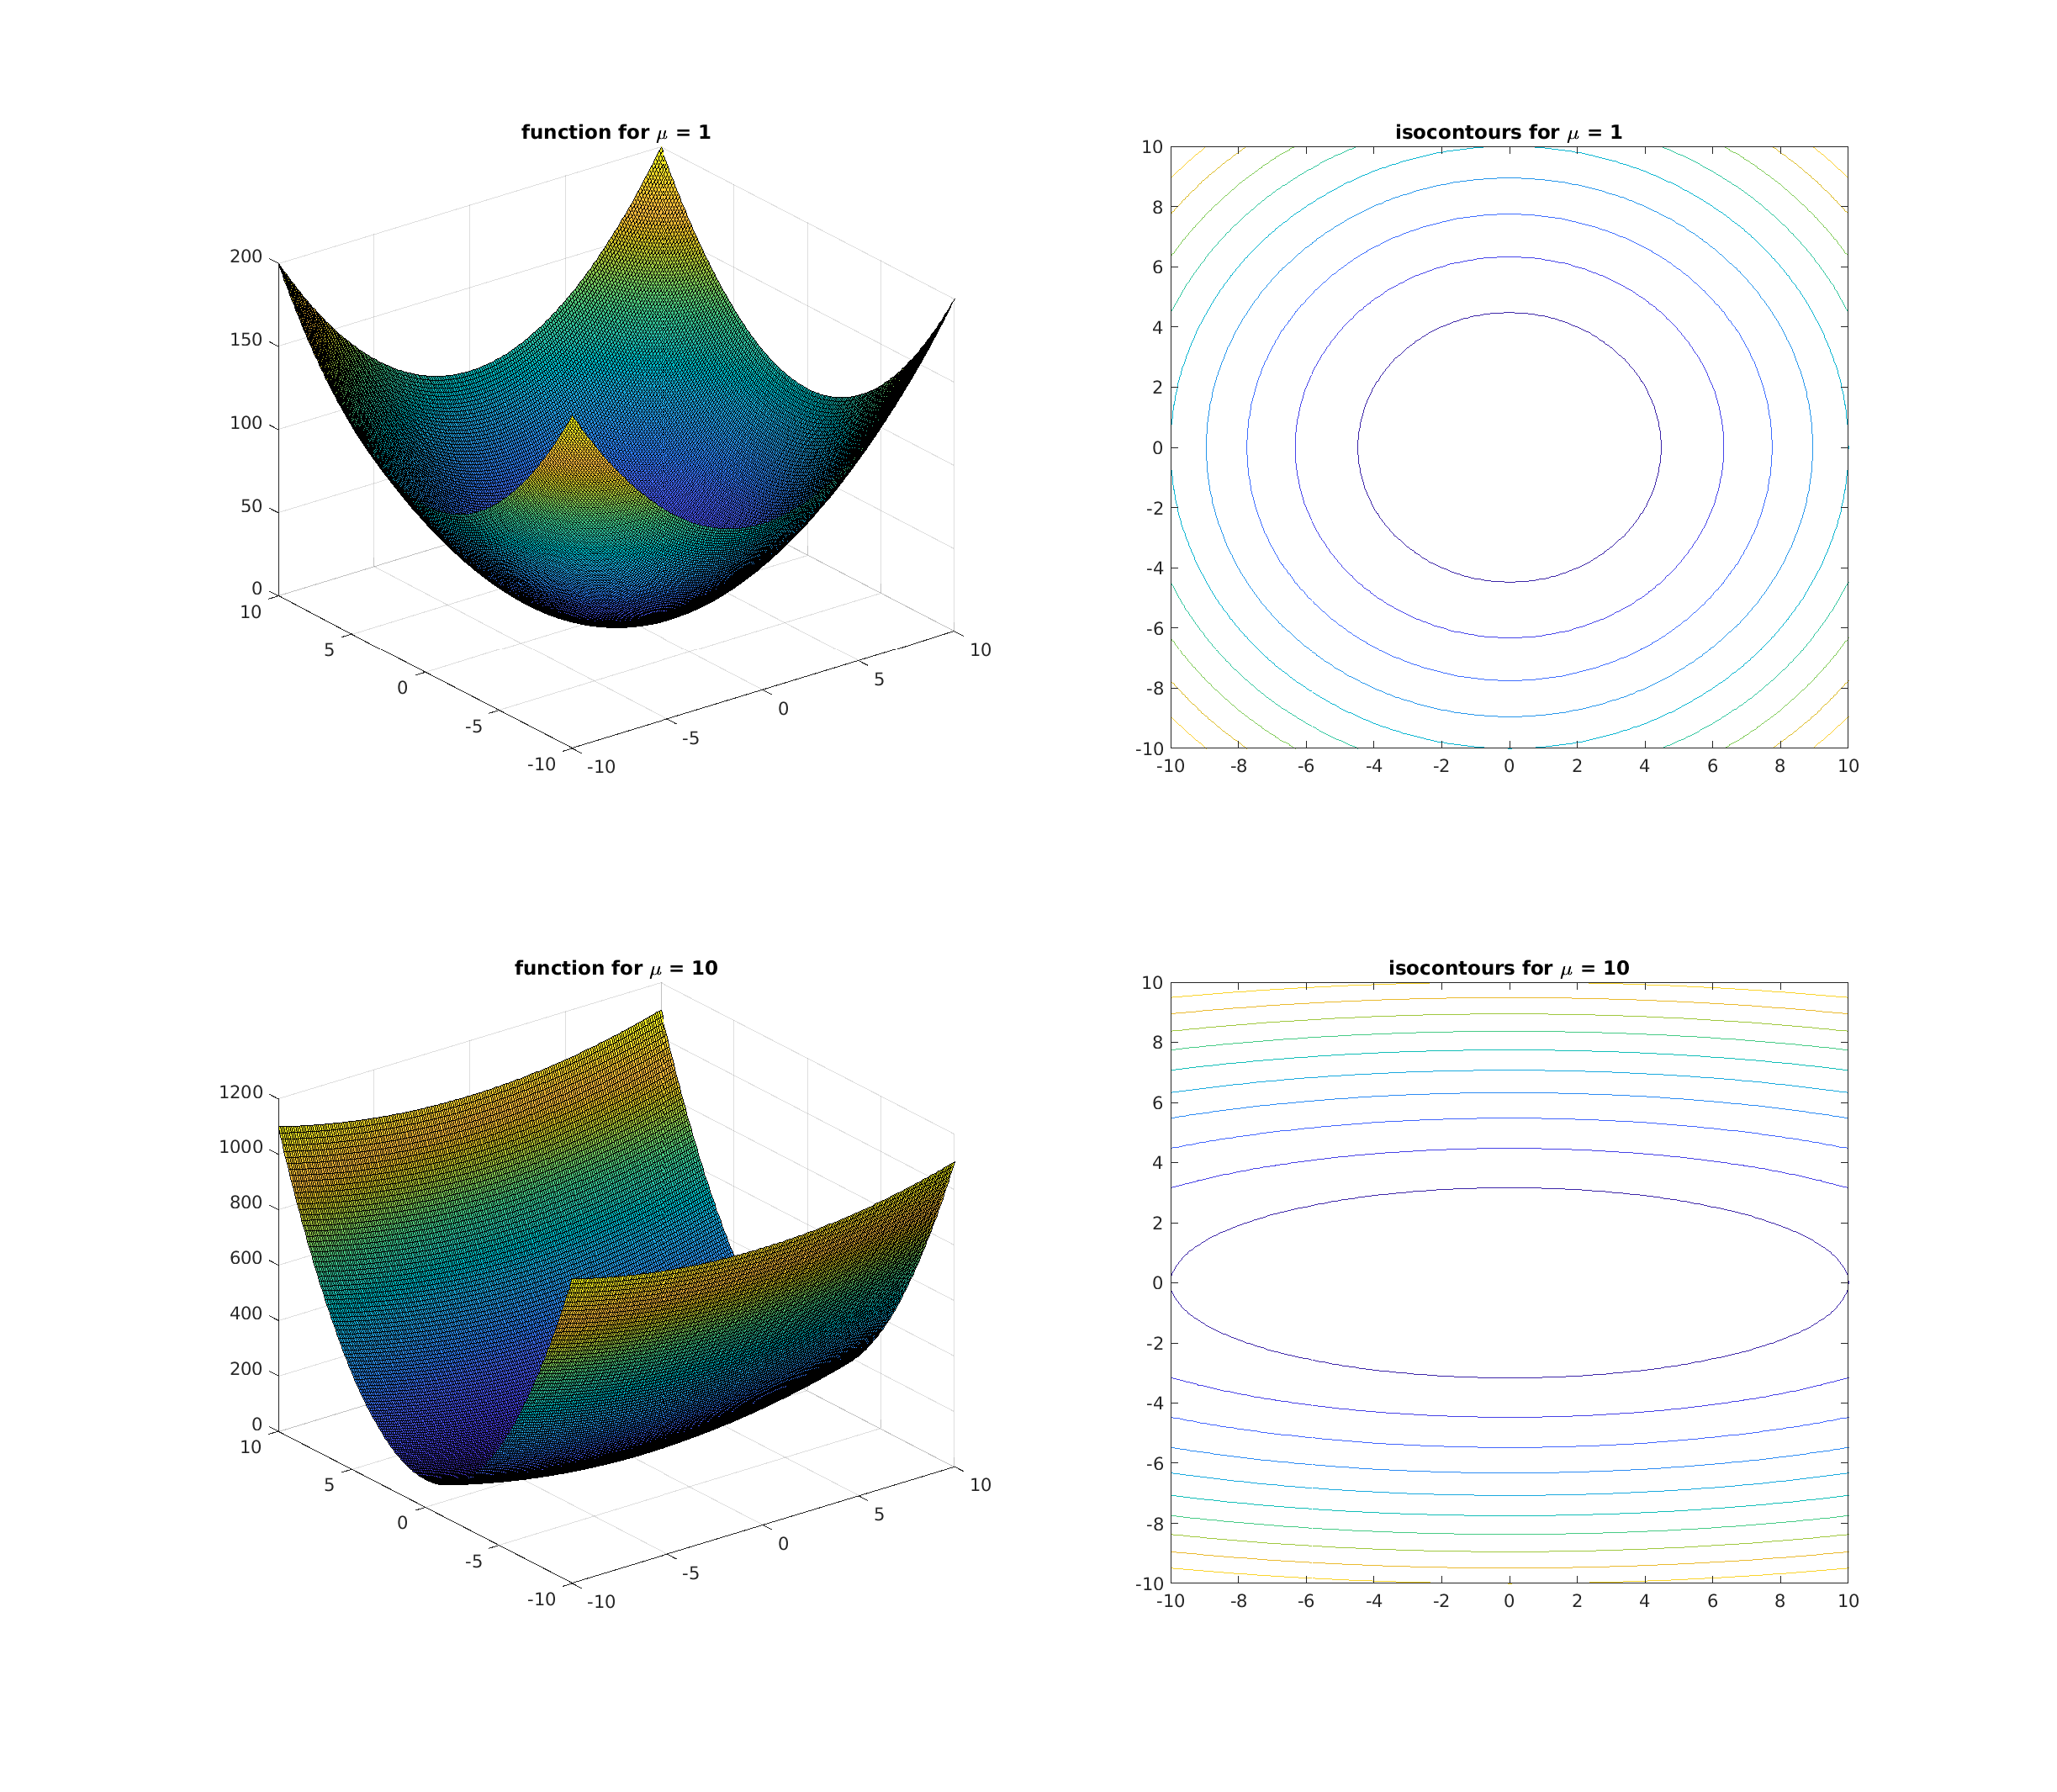
\includegraphics[width=\textwidth, trim={3cm 3cm 3cm 1cm}, clip]{./figures/ex3-2.eps}
\end{figure}

The matlab script is contained in \textit{code/ex3\_2.m} file. \newline
The behavior of the isolines $\propto \mu$ parameter that affects the steepness of the function in the y-dimension.
For $\mu = 1$, the isolines are circular, indicating that the function increases evenly in all directions from the origin.
A symmetric paraboloid from the origin is the result of our isotropic quadratic function where its coefficients
are equal, resulting in a radially symmetric growth.
For $\mu = 10$, the isolines are ellipses because the function grows faster on the y-dimension resulting in a paraboloid
steeper along the y-axis and flatter on the x-axis. 
This behavior is due to the scalar coefficient $\mu$.
Generally, the isolines indicates how the function behave in the space: 
closer contour lines mean that the function changes rapidly. 

\subsection{}
Considering that $A$ is a symmetric positive-definite matrix, find the exact optimal step-length $\alpha$.
Show your computations.\newline

Recalling the formula to compute the step length:
\myex{
    \alpha_k = \frac{\nabla f_k^T \nabla f_k}{\nabla f_k^T A \nabla f_k}
}
Note that $A$ is SPD $\therefore \, A = A^T$. 
$A = \myexthreeA$. $\nabla f_k = Ax - b = \myexthreeA \myvec{x \\ y}$ with $b = \vec{0}$. \newline
By plugging the previously obtained values into the definition:
\myex{
    \alpha_k 
    & = \frac{\nabla f_k^T \nabla f_k}{\nabla f_k^T A \nabla f_k} \\
    & = \frac{\myvec{x & y} \myexthreeA \myexthreeA \myvec{x \\ y}} 
            {\myvec{x & y} \myexthreeA \myexthreeA \myexthreeA \myvec{x \\ y}} \\
    & = \frac{4x^2 + 4 \mu^2 y^2}{8x^2 + 8 \mu^3 y^2} \\
    & = \frac{1}{2} \cdot \frac{x^2 + \mu^2 y^2}{x^2 + \mu^3 y^2} \\
    & = \alpha_{opt} \text{ for quadratic forms}
}
For $\mu = 1$:
\myex{
    \alpha_k 
    = \frac{1}{2} \cdot \frac{x^2 + y^2}{x^2 + y^2}
    = \frac{1}{2}
}
For $\mu = 10$:
\myex{
    \alpha_k 
    & = \frac{1}{2} \cdot \frac{x^2 + 100 y^2}{x^2 + 1000 y^2} \\
}

\subsection{}
Write a Matlab code for the gradient method with maximum number of iterations $N = 100$ and a tolerance $tol = 10-8$. 
Minimize $f$ for $\mu = (1, 10)$ and starting points: $(x_0 , y_0) = (10, 0), (0, 10), (10, 10)$.



\subsection{}
For each case plot the iterations on the energy landscape in 2D (the plot of the objective function),
the log10 of the norm of the gradient and the value of the energy function (objective function) as functions of the iterations. 
Comment the results.

\end{document}
